\documentclass{beamer}
\usepackage[utf8]{inputenc}
\usepackage[english,german]{babel} 
\usepackage{listings} 
\usepackage{listings-golang}
\usepackage[absolute,overlay]{textpos}
\usepackage{tcolorbox}

\usepackage[absolute,overlay]{textpos}
  \setlength{\TPHorizModule}{1mm}
  \setlength{\TPVertModule}{1mm}

\titlegraphic{
\includegraphics[scale=0.1]{golanglogo.png}}
\title{
	\Large{\textit{\\Die Programmiersprache Go - Eine Einf\"uhrung}} \\
	\Large{\textbf{\\Seminarvortrag}}
}
\author{Student: Adrian Helberg \\Prüfer: Prof. Dr. Axel Schmolitzky}
\date{\today}

\definecolor{mygreen}{rgb}{0,0.6,0}

\begin{document}
\lstset{
    frame=single,
    basicstyle=\footnotesize,
    keywordstyle=\color{blue},
    showstringspaces=false, 
    stringstyle=\color{mygreen},
    tabsize=4,
    language=Golang
}

\maketitle

\frame{\tableofcontents}

\begin{frame}

\begin{quote}
``Go is an open source programming language that makes it easy to build simple, reliable and efficient software." 
\end{quote}

\begin{flushright}
\scriptsize (Go Website: \href{golang.org}{golang.org})
\end{flushright}

\begin{quote}
Go ist eine Open-Source-Programmiersprache, die es einfach macht, einfache, zuverlässige und effiziente Software zu erstellen.
\end{quote}

\begin{flushright}
\scriptsize (Eigene \"Ubersetzung)
\end{flushright}

\end{frame}

%%%%%%%%%%%%%%%%%% GESCHICHTE %%%%%%%%%%%%%%%%%%

\section{Geschichte}

%%%%%%%%%%%%%%%%%% ENTWICKLER %%%%%%%%%%%%%%%%%%
\subsection{Entwickler}
\begin{frame}
\frametitle{Entwickler}

\begin{itemize}
\setlength{\itemsep}{24pt}
\item Konzipiert September 2007
\item Robert Griesemer, Rob Pike und Ken Thompson
\item Mitarbeiter von Google LLC \textregistered
\item Aus Frust heraus entstanden
\item \textit{``Complexity is multiplicative''} - Rob Pike
\end{itemize}

\end{frame}

%%%%%%%%%%%%%%%%%% ENTWURFSPHASE %%%%%%%%%%%%%%%%%%

\subsection{Entwurfsphase}
\begin{frame}
\frametitle{Entwurfsphase}

\begin{itemize}
\setlength{\itemsep}{40pt}
\item Ausdrucksstarke und effiziente Kombination aus Kompilierung und Ausf\"uhrung
\item Ähnlichkeiten mit C
\item Adaptiert gute Ideen aus einigen Programmiersprachen: \\
Pascal, Modula-2, Oberon, Oberon-2, Alef, ...
\end{itemize}

\end{frame}

\begin{frame}
\frametitle{Entwurfsphase}

\begin{figure}
\centering
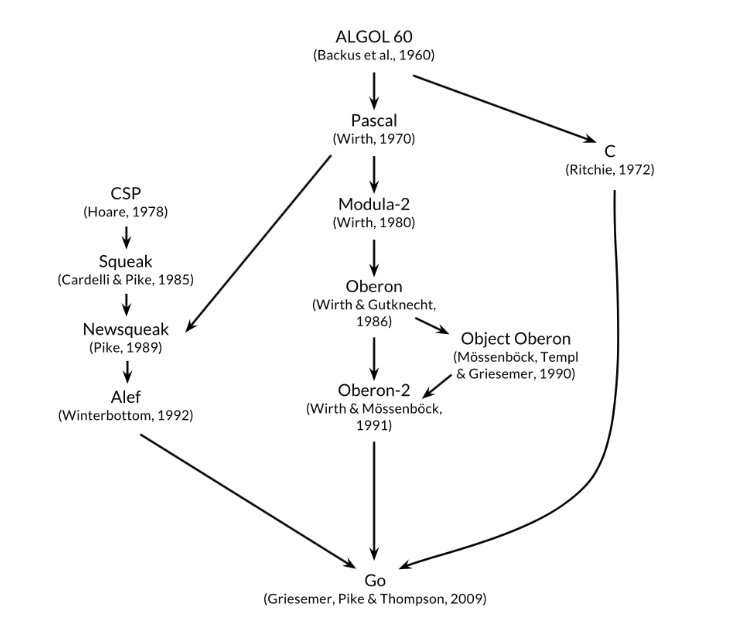
\includegraphics[scale=0.45]{origin.png}
\caption{The Go Programming Language,  Preface xii}
\end{figure}

\end{frame}

\begin{frame}
\frametitle{Entwurfsphase}

\begin{itemize}
\setlength{\itemsep}{40pt}
\item Vermeiden von features, die zu komplexen, unzuverl\"assigen code führen w\"urden
\item M\"oglichkeiten zur Nebenl\"aufigkeit sind neu und effizient
\item Datenabstraktion und Objektorientierung sind ungewohnt flexibel
\item Automatische Speicherverwaltung (garbage collection)
\end{itemize}

\end{frame}

%%%%%%%%%%%%%%%%%% VERÖFFENTLICHUNG %%%%%%%%%%%%%%%%%%

\subsection{Ver\"offentlichung}
\begin{frame}
\frametitle{Ver\"offentlichung}

\begin{itemize}
\setlength{\itemsep}{60pt}
\item Vorgestellt November 2009
\item Ber\"uhmt als Nachfolger für nicht typisierte Sriptsprachen
\begin{itemize}
\item[] $\rightarrow$ Verbindung aus Ausdruckskraft und Sicherheit
\end{itemize}
\end{itemize}

\end{frame}

%%%%%%%%%%%%%%%%%% GO-COMMUNITY %%%%%%%%%%%%%%%%%%

\subsection{Go-Community}
\begin{frame}
\frametitle{Go-Community}

\begin{itemize}
\setlength{\itemsep}{44pt}
\item Open-source projekt
\begin{itemize}
\item[] $\rightarrow$ Quellcode des Compilers, Bibliotheken (libraries) und Tools sind frei verfügbar
\end{itemize}
\item Aktive, weltweite Community
\item L\"auft auf Unix, Mac und Windows
\begin{itemize}
\item[] $\rightarrow$ \"Ublicherweise ohne Modifikation transpotrierbar
\end{itemize}
\end{itemize}

\end{frame}

%%%%%%%%%%%%%%%%%% MERKMALE UND SPRACHMITTEL %%%%%%%%%%%%%%%%%%

\section{Merkmale und Sprachmittel}

%%%%%%%%%%%%%%%%%% CLOSURES %%%%%%%%%%%%%%%%%%

\subsection{Closures}
\begin{frame}[fragile]
\frametitle{Closures}

Java
\lstset{language=Java, basicstyle=\scriptsize}
\begin{lstlisting}
private static Function<String, Supplier<String>> intSeq = 
x -> {

    AtomicInteger atomicInteger = new AtomicInteger();
    return () -> x + ": " + atomicInteger.incrementAndGet();
}

public static void main(String[] args) {

    Supplier<String> nextInt = intSeq.apply("Test 1");

    System.out.println(nextInt.get());
    System.out.println(nextInt.get());
}
\end{lstlisting}

\begin{textblock}{36}(88,66)
\begin{tcolorbox}
\textit{Ausgabe:\\}\\
Test 1: 1 \\
Test 1: 2
\end{tcolorbox}
\end{textblock}

\end{frame}

\begin{frame}[fragile]
\frametitle{Closures}

Go
\begin{lstlisting}
func intSeq(x string) func() string {
	i := 0
	return func() string {
		i++
		return x + ": " + strconv.Itoa(i)
	}
}

func main() {
	nextInt := intSeq("Test 1")

	fmt.Println(nextInt())
	fmt.Println(nextInt())
}
\end{lstlisting}

\begin{textblock}{36}(88,66)
\begin{tcolorbox}
\textit{Ausgabe:\\}\\
Test 1: 1 \\
Test 1: 2
\end{tcolorbox}
\end{textblock}

\end{frame}

\begin{frame}
\frametitle{Closures}

\begin{itemize}
\setlength{\itemsep}{24pt}
\item Philosophie: \textit{``Kommuniziere nicht, indem du Speicher teilst, sondern teile Speicher durch Kommunikation'}
\item Keine Einschr\"ankung beim Nutzen unsicherer Zugriffsmethode
\item \"Ublich: Goroutines, Channels
\begin{itemize}
\item Keine ``Race Conditions''
\end{itemize}
\end{itemize}

\end{frame}

\subsection{Reflection}
\begin{frame}[fragile]
\frametitle{Reflection}

Java
\lstset{language=Java, basicstyle=\scriptsize}
\begin{lstlisting}
public static String getStringProperty(Object object, 
                                        String methodname) {
    String value = null;

    try {
        Method getter = object.getClass()
                        .getMethod(methodname, new Class[0]);

        value = (String) getter
                        .invoke(object, new Object[0]);

    } catch (Exception e) {}

    return value;
}
\end{lstlisting}

\end{frame}

\begin{frame}[fragile]
\frametitle{Reflection}

Go
\begin{lstlisting}
func getField(v *Vertex, field string) int {

    r := reflect.ValueOf(v)
    f := reflect.Indirect(r).FieldByName(field)

    return int(f.Int())
}
\end{lstlisting}

\end{frame}

\begin{frame}
\frametitle{Reflection}

\begin{itemize}
\setlength{\itemsep}{24pt}
\item func ValueOf(i interface{}) Value
\begin{itemize}
\item Gibt ein Objekt Value (reflection interface) zurück, das auf den konkreten Wert initialisiert wurde, der in der Schnittstelle i gespeichert ist
\end{itemize}
\item func Indirect(v Value) Value
\begin{itemize}
\item Gibt den Wert zurück, auf den v zeigt
\end{itemize}
\item func (Value) FieldByName
\begin{itemize}
\item Gibt das \textit{struct field} mit dem angegebenen Namen zur\"uck
\end{itemize}
\item func (v Value) Int() int64
\begin{itemize}
\item Gibt den zugrunde liegenden Wert von v zur\"uck
\end{itemize}
\end{itemize}

\end{frame}

\subsection{Typsicherheit}
\begin{frame}
\frametitle{Typsicherheit}

\begin{itemize}
\setlength{\itemsep}{24pt}
\item Starke, statische Typisierung
\item Features simulieren dynamische Typisierung
\begin{itemize}
\setlength{\itemsep}{12pt}
\item Keine explizite Markierung von Interface-Implementierungen (Java: \textit{implements})
\item Stimmt eine Methodensignatur mit der des Interfaces \"uberein, wird diese automatisch implementiert (\"ahnlich: \textit{duck-typing})
\item Einfaches Erweitern externer Methoden (Library Funtionen)
\end{itemize}
\item OOP durch \textit{struct} und \textit{interface} m\"oglich
\end{itemize}

\end{frame}

\subsection{Objektorientierung}
\begin{frame}[fragile]
\frametitle{Objektorientierung}

\begin{itemize}
\item Typ \textit{struct}
\begin{itemize}
\setlength{\itemsep}{12pt}
\item Sammlung von Variablen und Funktionen
\item Methoden nicht virtuell
\item Man spricht bei Funktionen von \textbf{Methoden} durch Zugeh\"origkeit des \textit{structs}
\item Konvention: Nutzen von Zeigern bei ``Settern'',\\ \textit{Call-by-Value} bei ``Gettern''
\end{itemize}
\end{itemize}

\begin{lstlisting}
func (c *Circle) Enlarge() {
  c.radius += 1
}
\end{lstlisting}

\end{frame}

\begin{frame}[fragile]
\frametitle{Objektorientierung}

\begin{itemize}
\item Typ \textit{interface}
\begin{itemize}
\setlength{\itemsep}{12pt}
\item Virtuell
\item Objekt vom Typ \textit{Circle} kann einer Variable vom Typ \textit{Shape} zugeordnet werden, weil \textit{Circle} die notwendige Funktion \textbf{Area} bietet
\item Beliebig viele Interfaces!
\end{itemize}
\end{itemize}

\begin{lstlisting}
type Shape interface {
  Area() float64
}

func main() {
  var shape Shape = Circle{2}
  fmt.Println(shape.Area())
}
\end{lstlisting}

\end{frame}

\begin{frame}[fragile]
\frametitle{Objektorientierung}

\begin{itemize}
\item Polymorphie
\end{itemize}

\begin{lstlisting}
type Shape interface {
  Area() float64
}

func (c Circle) Area() float64{
  return math.Pi * c.radius * c.radius
}

func (r Rectangle) Area() float64{
  return r.length * r.width
}
\end{lstlisting}

\end{frame}

\subsection{Speicherbereinigung}
\begin{frame}
\frametitle{Speicherbereinigung}

\begin{itemize}
\setlength{\itemsep}{30pt}
\item Automatisch
\item \textit{Garbage Collector}
\item Wird eine Variable unerreichbar, wird sie recyklet
\end{itemize}

\end{frame}

\section{Docker}
\begin{frame}

\frametitle{Docker}

\begin{itemize}
\setlength{\itemsep}{12pt}
\item Open-Source Apache 2.0 Lizens
\item Basiert auf \textit{Namespaces}
\item Isolierung von Anwendungen mit Containervirtualisierung
\item Ressourcentrennung (Code, Laufzeitmodul, Systemwerkzeuge, Systembibliotheken, ...)
\item Offiziell von der IANA zugewiesene Portnummern 2375 für HTTP- und 2376 für HTTPS-Kommunikation
\item Erstellung von Containern mit virtuellen Betriebssystemen
\end{itemize}

\begin{textblock}{20}(84,0)

\includegraphics[scale=0.22]{docker.png}
\end{textblock}

\end{frame}

\begin{frame}

\frametitle{Docker}

\begin{itemize}
\setlength{\itemsep}{20pt}
\item Docker Hub als Online-Dienst als Verteiler fest integriert
\item Eingebaute Versionsverwaltung, angelehnt an
\end{itemize}

\begin{textblock}{20}(84,0)

\includegraphics[scale=0.22]{docker.png}
\end{textblock}

\begin{textblock}{20}(92,49)

\includegraphics[scale=0.22]{gitlogo.png}
\end{textblock}

\end{frame}

\section{Zentrale Fragestellung}
\begin{frame}
\frametitle{Zentrale Fragestellung}

\centering
\glqq flexibel wie dynamisch getyped,\\ aber mit statischer Typsicherheit?\grqq{}

\end{frame}

\section{Pro \& Contra}
\begin{frame}
\frametitle{Pro \& Contra}

\begin{tabular}{p{5cm} | p{5.5cm}}
\textbf{Pro} & \textbf{Contra} \\ \hline
\begin{itemize}
\setlength{\itemsep}{20pt}
\item Minimalismus
\item Statisches Duck-Typing
\item Parallelisierung
\item Aufger\"aumte Syntax
\item Schneller Compiler
\end{itemize}
&
\begin{itemize}
\setlength{\itemsep}{20pt}
\item Keine generische Programmierung
\item nil statt Option
\item Wenig grundlegende Datenstrukturen
\item Keine Methodenüberladung
\end{itemize}
\\
\end{tabular}

\end{frame}

\begin{frame}
\frametitle{Pro \& Contra}

\begin{tabular}{p{5cm} | p{5.5cm}}
\textbf{Pro} & \textbf{Contra} \\ \hline
\begin{itemize}
\setlength{\itemsep}{20pt}
\item Statisch gelinkte Binärdateien
\item Laufzeiteigenschaften
\item Integriertes Unit-Test-Framework
\item Paketmanager
\end{itemize}
&
\begin{itemize}
\setlength{\itemsep}{20pt}
\item Unbefriedigende API-Dokumentation
\item Teilweise umständliche APIs
\item Umst\"andliches Mocking
\item Kleines \"Okosystem
\end{itemize}
\\
\end{tabular}

\end{frame}

\section{Compiler}
\begin{frame}
\frametitle{Compiler}

\begin{itemize}
\setlength{\itemsep}{20pt}
\item Gc
\item Gccgo
\end{itemize}

\end{frame}

\section{Einzelnachweise}
\begin{frame}
\frametitle{Einzelnachweise}

\begin{itemize}
\setlength{\itemsep}{20pt}
\item ...
\end{itemize}

\end{frame}

\end{document}